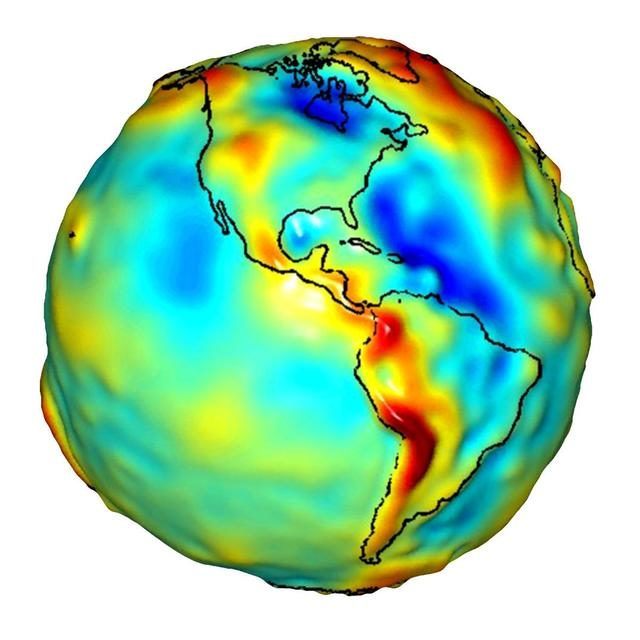
\includegraphics[height=1.25cm]{images/pictograms/gravity}

\includegraphics[height=1.25cm]{images/pictograms/benchmark}

\includegraphics[height=1.25cm]{images/pictograms/3d}

%%%%%%%%%%%%%%%%%%%%%%%%%%%%%%%%%%%%%%%%%%%%%%%%%%%%%%%%%%%%%%%%%%%%%%%%%%%%%%%%%%%%%%%%%%%%%%%%%%%

\lstinputlisting[language=bash,basicstyle=\small]{python_codes/fieldstone_84/keywords.ascii}

\begin{center}
Code at \url{https://github.com/cedrict/fieldstone/tree/master/python_codes/fieldstone_84}
\end{center}

\par\noindent\rule{\textwidth}{0.4pt}

{\sl This stone was developed in collaboration wth Sverre Hassing}. \index{contributors}{S. Hassing}

\par\noindent\rule{\textwidth}{0.4pt}
%%%%%%%%%%%%%%%%%%%%%%%%%%%%%%%%%%%%%%%%%%%%%%%%%%%%%%%%%%%%%%%%%%%%%%%%%%%%%%%%%%%%%%%%%%%%%%

This stone deals with the forward calculations of gravity fields (potential, vector and tensor).
It implements to different ways: 
\begin{itemize}
\item the point mass approach: each cell of size $(h_x,h_y,h_z)$ and of constant density $\rho$
is contracted to a single point in its middle of equivalent mass $m=\rho h_xh_yh_z$.
\item the prism approach, as explained in Appendix~\ref{MMM-app:prisms}.
\item the Gauss quadrature approach using $n_q^3$ points per cell.
\end{itemize}

Three types of gravity measurements are implemented:
\begin{itemize}
\item on a plane, defined by z=z\_{plane}, of size $Lx \times Ly$, counting nnx\_plane X nny\_plane points
\item on a line, starting at point (x\_begin,y\_begin,z\_begin) and ending at point (x\_end,y\_end,z\_end)
\item at a single point, atcoordinates xpt,ypt,zpt from the center of the object
\item on a 3D spiral starting at the north pole and going to the south pole, parameterised only 
by the total number of points and the distance to the center/radius of all spiral points.
This is called the Fibonacci spiral, or lattice on a sphere. The code is borrowed from the 
one in the gravity post-processor of ASPECT.
\end{itemize}

We will try to answer those questions:
Is it worth using prisms instead of mass points ?  
If so, how much more accurate are the former than the latter?
How much more expensive in terms of cpu time are prism-based calculations ?
What about the Gauss quadrature approach ? 

The domain is a cuboid of size $L_x\times L_y \times L_z$ cut into $nel_x \times nel_y \times nel_z=nel$ cells.
Note that in all what follows a cell has a constant density. 

The function {\tt grav\_calc} computes $u$, $\vec{g}$ and ${\bm T}$ using one of the 
three methods hilighted above. 

Note that the \aspect postprocessor relies on the Gauss-Legendre quadrature, 
see also \textcite{vohb81} (1981).

\newpage
%-------------------------------
\subsection*{Buried sphere}

The domain is a cube of $L=1\si{\km}$ size. All elements inside a sphere of radius $R=L/2$ are assigned
$\rho_s=100\si{\kg\per\cubic\metre}$.
The mass of the sphere is 
\[
M_s = \frac{4}{3}\pi R^3 \rho \simeq 5.23598775598 \cdot 10^{10} \si{kg}
\]
So that outside of the sphere the gravity field and potential are trivial to compute:
\[
|\vec{g}(r)|={\cal G}\frac{M_s}{r^2}
\qquad
\qquad
U(r)={\cal G}\frac{M_s}{r}
\]
Gravity terms are computed on a line starting at $\vec{r}=(0,0,0)$ and ending at $\vec{r}=(1.11,2.22,5.55)\si{km}$ (this is to avoid any cancelling due to symmetry).
The analytical expressions for the gravity and gravity potential are 
\begin{eqnarray}
|\vec{g}(r)|=g(r) 
&=& {\cal G} \rho \frac{4}{3}\pi r \qquad \text{inside} \nn\\
&=& {\cal G} \rho \frac{4}{3}\pi \frac{R^3}{r^2}  \qquad \text{outside} \nn\\
U(r) 
&=& - 2 \pi {\cal G} \rho (R^2-r^2/3) \qquad \text{inside} \nn\\
&=& - {\cal G} \rho \frac{4}{3}\pi \frac{R^3}{r}  \qquad \text{outside} \nn
\end{eqnarray}

\begin{center}
\includegraphics[width=8cm]{python_codes/fieldstone_84/sphere/setup}
\end{center}


\begin{center}
\includegraphics[width=8cm]{python_codes/fieldstone_84/sphere/gravnorm}
\includegraphics[width=8cm]{python_codes/fieldstone_84/sphere/gravpot}\\
\includegraphics[width=8cm]{python_codes/fieldstone_84/sphere/gravnorm_error}
\includegraphics[width=8cm]{python_codes/fieldstone_84/sphere/gravpot_error}\\
{\captionfont  The grey area indicates the sphere. Mesh resolution?}
\end{center}

The gravity was also measured at location $(123,234,345)\si{\metre}$ counted from the center of the sphere
for increasing resolutions. 

\begin{center}
\includegraphics[width=8cm]{python_codes/fieldstone_84/sphere/single_point_g.pdf}
\includegraphics[width=8cm]{python_codes/fieldstone_84/sphere/single_point_U.pdf}\\
\includegraphics[width=8cm]{python_codes/fieldstone_84/sphere/single_point_g_error.pdf}
\includegraphics[width=8cm]{python_codes/fieldstone_84/sphere/single_point_U_error.pdf}
\end{center}


\newpage
%-------------------------------
\subsection*{Buried cube}

The domain is a cube of $L=1\si{\km}$ size. All elements inside a cube of size $d=L/8$ are assigned
$\rho_s=100\si{\kg\per\cubic\metre}$.
The mass of the cube is then
\[
M_c = \rho d^3 = 1.95312500\cdot 10^8 \si{\kg}
\]
Far away from the cube $g(r) \rightarrow {\cal G}M_c \rho/r^2$ and $U(r) \rightarrow -{\cal G} M_c/r$.

\begin{center}
\includegraphics[width=6cm]{python_codes/fieldstone_84/cube/setup}
\end{center}


\begin{center}
\includegraphics[width=7cm]{python_codes/fieldstone_84/cube/gravnorm}
\includegraphics[width=7cm]{python_codes/fieldstone_84/cube/gravpot}\\
\includegraphics[width=5cm]{python_codes/fieldstone_84/cube/tensor_xx}
\includegraphics[width=5cm]{python_codes/fieldstone_84/cube/tensor_yy}
\includegraphics[width=5cm]{python_codes/fieldstone_84/cube/tensor_zz}\\
\includegraphics[width=5cm]{python_codes/fieldstone_84/cube/tensor_xy}
\includegraphics[width=5cm]{python_codes/fieldstone_84/cube/tensor_xz}
\includegraphics[width=5cm]{python_codes/fieldstone_84/cube/tensor_yz}\\
{\captionfont  The grey area indicates the sphere. resolution $32\times 32 \times 32$.}
\end{center}

\begin{center}
\includegraphics[width=5cm]{python_codes/fieldstone_84/cube/g}
\includegraphics[width=5cm]{python_codes/fieldstone_84/cube/U}
\includegraphics[width=5cm]{python_codes/fieldstone_84/cube/horgrad}
\end{center}

\begin{center}
\includegraphics[width=5cm]{python_codes/fieldstone_84/cube/Txx}
\includegraphics[width=5cm]{python_codes/fieldstone_84/cube/Tyy}
\includegraphics[width=5cm]{python_codes/fieldstone_84/cube/Tzz}\\
\includegraphics[width=5cm]{python_codes/fieldstone_84/cube/Txy}
\includegraphics[width=5cm]{python_codes/fieldstone_84/cube/Txz}
\includegraphics[width=5cm]{python_codes/fieldstone_84/cube/Tyz}\\
{\captionfont  xxx}
\end{center}

The gravity was also measured at location $(12,23,34)\si{\metre}$ counted from the center of the cube
for increasing resolutions. 

\begin{center}
\includegraphics[width=8cm]{python_codes/fieldstone_84/cube/single_point_g.pdf}
\includegraphics[width=8cm]{python_codes/fieldstone_84/cube/single_point_U.pdf}\\
\includegraphics[width=8cm]{python_codes/fieldstone_84/cube/single_point_g_error.pdf}
\includegraphics[width=8cm]{python_codes/fieldstone_84/cube/single_point_U_error.pdf}\\
\end{center}


\newpage
%-------------------------------
\subsection*{Salt diapir}


The domain has dimensions $L_x=2940$, $L_y=2100$, $L_z=3060$ and the data set makes that  
nelx=98, nely=70 and nelz=153. The data is
synthetically generated using methods described in \textcite{clcc19} (2019)
and the file containing the data is {\sl salt\_dome.data}.
The salt has a relative density of $-400\si{\kg\per\cubic\metre}$.

\begin{center}
\includegraphics[width=10cm]{python_codes/fieldstone_84/diapir/diapir.png}
\end{center}

\begin{center}
\includegraphics[width=5cm]{python_codes/fieldstone_84/diapir/g.png}
\includegraphics[width=5cm]{python_codes/fieldstone_84/diapir/U.png}
\includegraphics[width=5cm]{python_codes/fieldstone_84/diapir/horgrad.png}\\
{\captionfont gravity vector norm, gravity potential, and horizontal gradient}
\end{center}


%------------------------------------------
\subsection*{Prism of Arroyo et al (2015)}

\begin{center}
\includegraphics[width=8cm]{python_codes/fieldstone_84/arct15/setup}
\includegraphics[width=8cm]{python_codes/fieldstone_84/arct15/arct15.png}\\
{\captionfont Left: setup. Right: taken from \textcite{arct15} (2015).}
\end{center}


\begin{center}
\includegraphics[width=5.3cm]{python_codes/fieldstone_84/arct15/g.png}
\includegraphics[width=5.3cm]{python_codes/fieldstone_84/arct15/U.png}
\includegraphics[width=5.3cm]{python_codes/fieldstone_84/arct15/horgrad.png}\\
\includegraphics[width=5.3cm]{python_codes/fieldstone_84/arct15/Txx}
\includegraphics[width=5.3cm]{python_codes/fieldstone_84/arct15/Tyy}
\includegraphics[width=5.3cm]{python_codes/fieldstone_84/arct15/Tzz}\\
\includegraphics[width=5.3cm]{python_codes/fieldstone_84/arct15/Txy}
\includegraphics[width=5.3cm]{python_codes/fieldstone_84/arct15/Txz}
\includegraphics[width=5.3cm]{python_codes/fieldstone_84/arct15/Tyz}\\
{\captionfont gravity vector norm, gravity potential, horizontal gradient,
and 6 components of ${\bm T}$.}
\end{center}


%------------------------------------------
\subsection*{Whole Earth with PREM density}

\index{general}{P.R.E.M.}

\begin{center}
\includegraphics[width=8cm]{python_codes/fieldstone_84/earth/setup}
\includegraphics[width=8cm]{python_codes/fieldstone_84/earth/rho}\\
{\captionfont resolution $150\times 150 \times 150$. Density is obtained from the PREM model \cite{dzan81}.}
\end{center}


\begin{center}
\includegraphics[width=7cm]{python_codes/fieldstone_84/earth/gravnorm}
\includegraphics[width=7cm]{python_codes/fieldstone_84/earth/gravpot}\\
{\captionfont resolution $64 \times 64 \times 64$.}
\end{center}

\begin{center}
\includegraphics[width=7cm]{python_codes/fieldstone_84/earth/spiral.png}\\
{\captionfont Spiral of 500 points at height $250~\si{\km}$ above the Earth surface. 
Earth is ased on $64\times 64 \times 64$ resolution.}
\end{center}


%------------------------------------------
\subsection*{Hollow Earth with constant density}

The density is constant and set to $\rho=4000\si{\kg\per\cubic\metre}$. 
Outer radius is $6371~\si{\km}$ and inner radius is $3480~\si{\km}$.

%\begin{center}
%\includegraphics[width=8cm]{python_codes/fieldstone_84/hollow_earth/setup}
%\includegraphics[width=8cm]{python_codes/fieldstone_84/hollow_earth/rho}\\
%{\captionfont resolution 150x150x150. }
%\end{center}

\begin{center}
\includegraphics[width=7cm]{python_codes/fieldstone_84/hollow_earth/gravnorm}
\includegraphics[width=7cm]{python_codes/fieldstone_84/hollow_earth/gravpot}\\
{\captionfont resolution $64 \times 64 \times 64$}
\end{center}










